
\section{Background}

\subsection{Convolution Operations}

At the convolutional stage, the computational kernel takes as input a batch of 2D multi-channel feature maps and a bank of  2D
multi-channel filters. The computation produces a batch of 2D multi-channel output feature maps with the same batch size as input. To
compute one output feature map, all filters are used to convolve with the same input feature map. Specifically, each filter slides over the
input feature map to perform an elementwise multiplication with the part of input where it is currently located and then sums up the
results across all channels.

\begin{figure}
\centering
  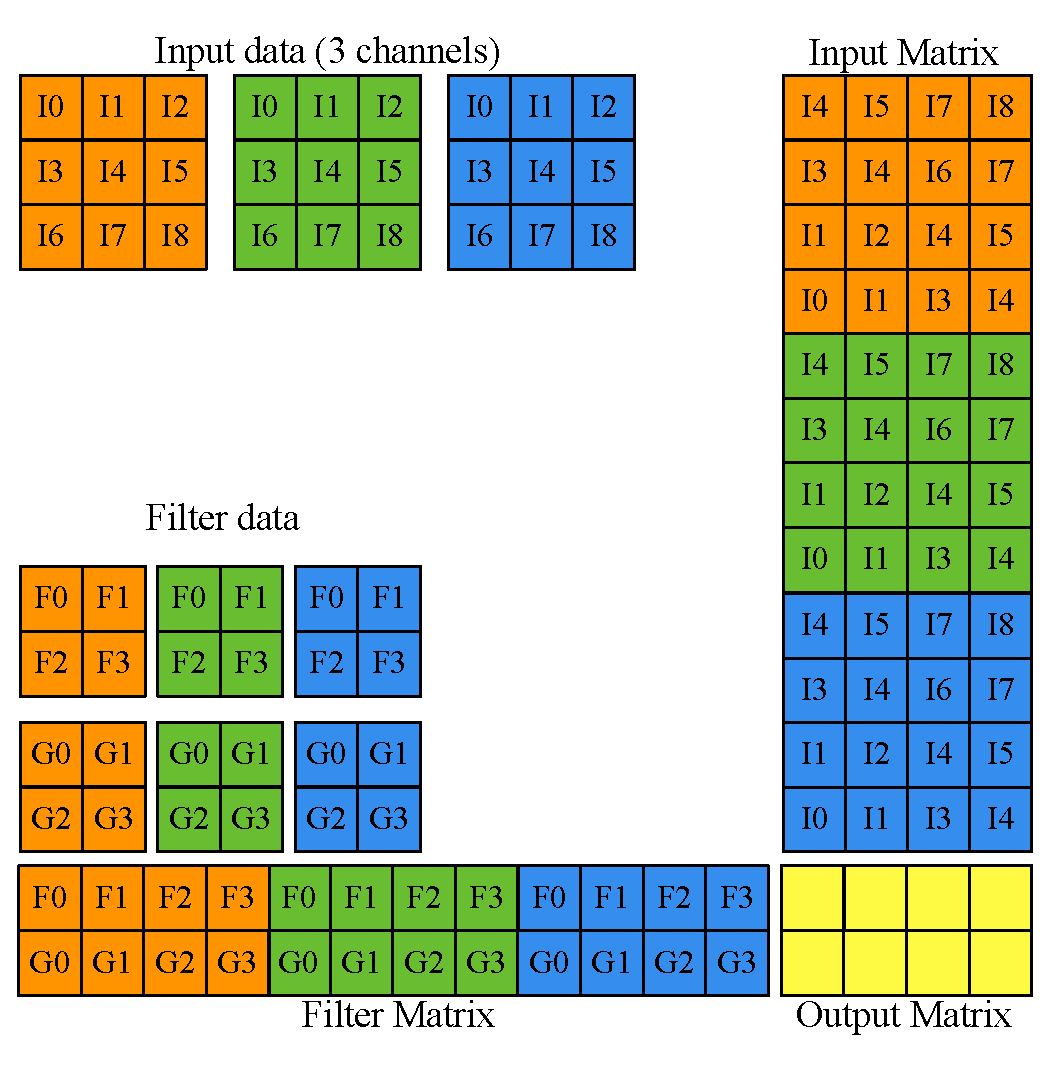
\includegraphics[width=0.75\columnwidth,height=6cm]{./figure/convlowering.eps}
  \caption{An example (reproduced from \cite{ChetlurWVCTCS14}) of converting a simple convolution into matrix multiplications. Here, two filters are used to convolve with a 3-channel input.}
  \label{fig:convlowering}
\end{figure}

Representative algorithms for convolution operations, including GEMM-, FFT- and Winograd-based convolutions, all require to transform 4D
tensors into a transformed matrix where computation can be performed. Doing so can incur high memory overhead. For example, Figure
\ref{fig:convlowering} illustrates the process of GEMM-based convolution where two filters are applied to a 3-channel input data. All data
are organized as a 4-element tuple, $(batch\_size, channel\_size, height, width)$. The dimension of the filter data in Figure
\ref{fig:convlowering} is $(2, 3, 2, 2)$. The transformed filter matrix has the same number of elements as the filter data. The input data
are of size $(1, 3, 3, 3)$ and have 27 elements in total. However, after transforming the input data into an input matrix, the resulting
matrix would have 48 elements, 44\% of which are redundant elements. This can incur redundant memory accesses for loading and storing the
matrix elements. Our work aims to eliminate the redundant elements to reduce the overhead for memory accessing. 



%\subsection{Overview of Our Approach}
\begin{figure}[t!]
\centering
  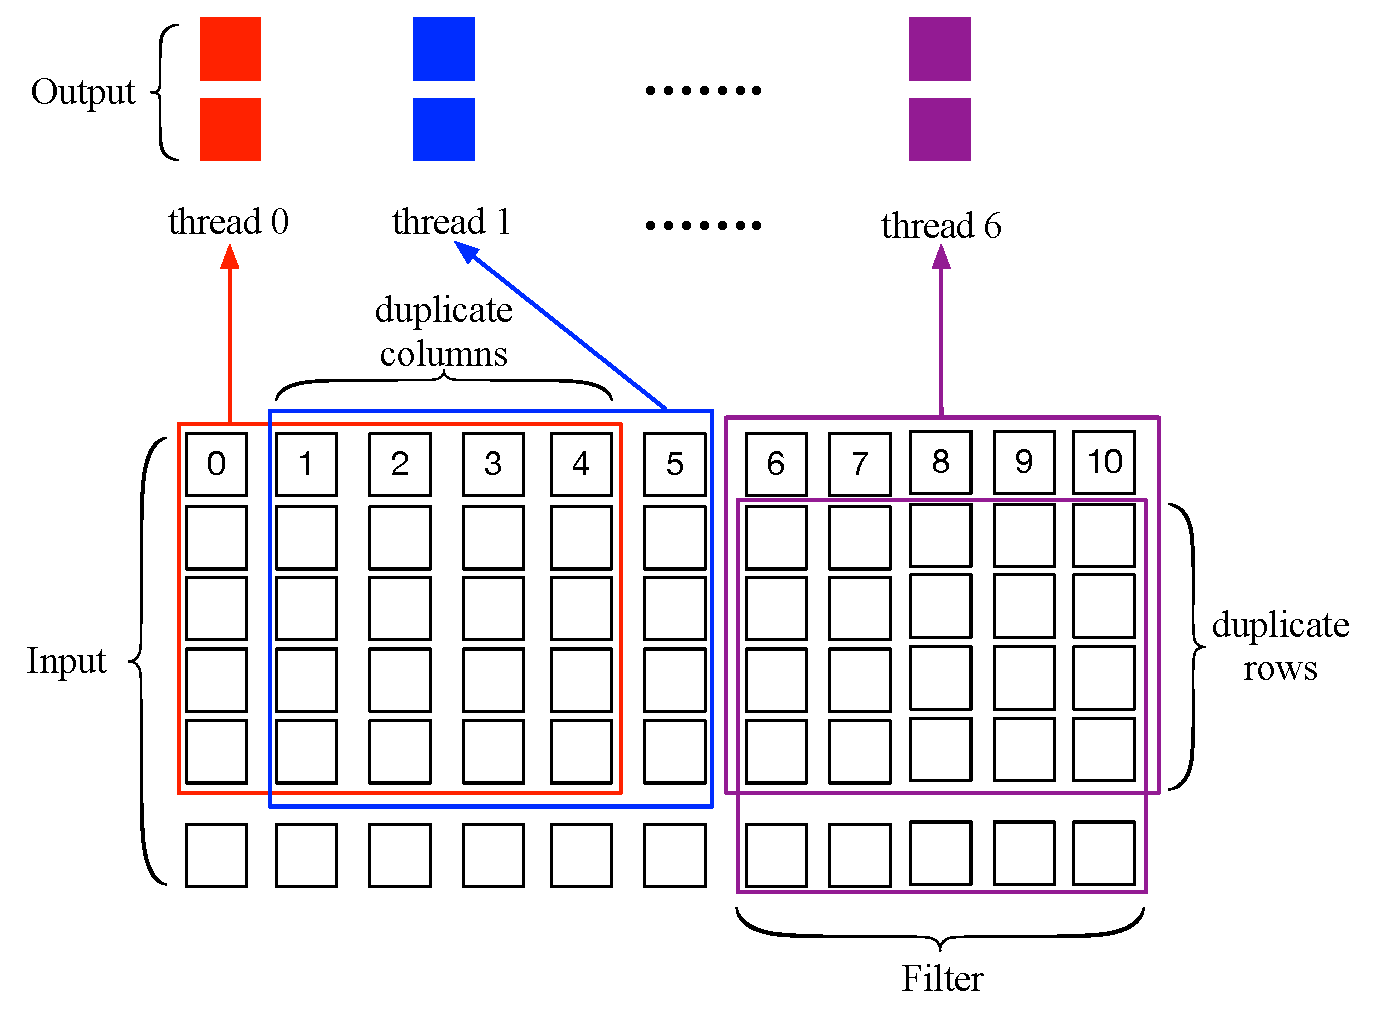
\includegraphics[width=\columnwidth,height=6cm]{./figure/twostrategies.eps}
  \caption{Example of performing 2D convolution using a GPU. Here, the filter size is $5 \times 5$, the input image size is $6 \times 11$
  and the output size is $2 \times 7$. Each thread calculates one column of the output. Assume threads 0 and 1 load the required regions from input
  image with four duplicate columns, and thread 6 loads two overlapped regions from input image and generates four duplicate rows. Numbers in
  the square denote the index of input elements.}
  \label{fig:twostrategies}
\end{figure}
